\documentclass[pra,12pt]{revtex4}
\usepackage{amsmath}
\usepackage{amssymb}
\usepackage{graphicx}
\usepackage{color}
\usepackage[pdfborder={0 0 0},colorlinks=true,linkcolor=blue]{hyperref}

\def\ket#1{\left|#1\right\rangle}
\def\bra#1{\left\langle#1\right|}
\def\braket#1{\left\langle#1\right\rangle}

\setlength{\parindent}{0pt}

\renewcommand{\baselinestretch}{1.0}
\setlength{\parskip}{0.07in}

\begin{document}

\section{Bound states and extended states}

One of the most interesting features of wavefunctions in infinite
space is that they come in two distinct types: (i) \textbf{extended
  states}, which spread out over the entire space, and (ii)
\textbf{bound states}, which are localized in one region.  Both types
can co-exist in a single system.

The \textbf{1D finite square well} is a simple model which exhibits
both bound and extended states.  Consider the Hamiltonian
$$\hat{H} = \frac{\hat{p}^2}{2m} - V_0 \,\Theta(a -|\hat{x}|),$$ where
$\hat{x}$ and $\hat{p}$ are the 1D position and momentum operators,
$m$ is the particle mass, $V_0$ and $a$ are positive real parameters,
and $\Theta(\cdots)$ denotes the Heaviside step function (which is 1
if the input is positive, and 0 otherwise).  The potential describes a
square well of depth $V_0$ and width $2a$.  Inside the well region
($|x| < a$), the potential is $-V_0$; outside, it is zero.

\begin{figure}[h]
  \centering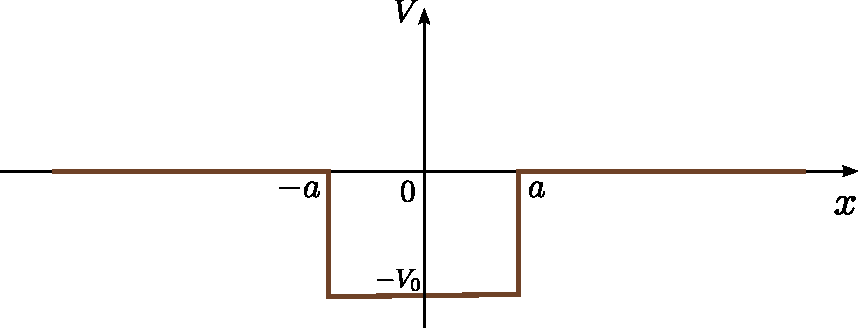
\includegraphics[width=0.7\textwidth]{squarewell}
\end{figure}

We wish to solve the time-independent Schr\"odinger equation for this
Hamiltonian.  In \hyperref[sec:appendix]{Appendix A}, we describe a
common numerical method, known as the \textbf{transfer matrix method},
which can be used to generate solutions for the square well and other
similar 1D potentials.  In this section, we not deal with the
calculation details, but instead zoom in on certain key facts.

The first thing to note is that when solving the Schr\"odinger wave
equation, it's necessary to specify the boundary conditions at
infinity.  This choice affects whether we get a bound state or
extended state.  The wavefunction of a bound state diminishes
exponentially as $x \rightarrow \pm\infty$; thus, in either external
region (i.e., $x < -a$ or $x > a$), it satisfies
$$-\frac{\hbar^2}{2m}\,\frac{d^2\psi}{dx^2} = E \psi(x),$$
subject to the boundary conditions
$$\psi(x) \overset{x\rightarrow\pm\infty}{\sim} e^{\mp\kappa x}, \;\;\;\mathrm{Re}(\kappa) > 0.$$
The bound state solutions in the external regions therefore take the
form
$$\psi(x) = c_\pm\, e^{\mp\kappa x}, \;\;\mathrm{where}\;\, -\frac{\hbar^2\kappa^2}{2m} = E, \;\; c_\pm \in \mathbb{C}.$$
Since $E$ is real, it follows that $\kappa$ is real, and hence $E <
0$.  Moreover, the variational principle implies that $E \ge -V_0$.
Hence, bound state energies are restricted to the range $-V_0 \le E <
0$.  We can also show that the bound state energies are
\textit{discrete}: the energy spacing decreases with $a$, but so long
as $a$ is finite, the spacing is non-vanishing.  Another related
fact is that the wavefunction for a bound state can always be
normalized:
$$\int_{-\infty}^\infty |\psi(x)|^2\, dx\; =\; 1.$$
The normalization integral will not diverge, as $|\psi(x)|^2$ vanishes
exponentially as $x \rightarrow \pm \infty$.

For an extended state, the situation is quite different.  In this
case, the wavefunction does not vanish exponentially at infinity, but
instead takes the form
$$\psi(x) = \begin{cases} \alpha_-\, e^{ik x} + \beta_-\, e^{-ik x}, & \;\;\;x < -a\\ (\mathrm{something}) , & -a < x < a\\ \alpha_+\, e^{ik x} + \beta_+\, e^{-ik x} , & \;\;\,x > a.\end{cases}$$
Within each external region, $\psi(x)$ consists of a superposition of
left-moving and right-moving plane waves, with wavenumber $k$.  The
coefficients $\alpha_\pm$ and $\beta_\pm$ are not independent
quantities, but are linked by a linear relation (see
\hyperref[sec:appendix]{Appendix A}).  In order to satisfy
Schr\"odinger's equation, $k$ must satisfy
$$\frac{\hbar^2k^2}{2m} = E,$$
which means that extended states occur only for energies $E \ge 0$.
In fact, the solutions form a continuum, meaning we can find extended
states for \textit{every} $E \ge 0$.  Since $|\psi(x)|^2$ does not
diminish exponentially at infinity, $\int_{-\infty}^\infty
|\psi(x)|^2\, dx$ is necessarily a divergent integral (except in the
trivial case where the integrand is zero).  Hence, the wavefunction
has no finite normalization.  (Note: we formally exclude the case of
wavefunctions that blow up at infinity, rather than going to a
constant magnitude.  To understand why, and for a more rigorous
discussion of how extended states are normalized, see
\hyperref[sec:normalization]{Appendix B}.)

The results for the square well are summarized in the following figure:

\begin{figure}[h]
  \centering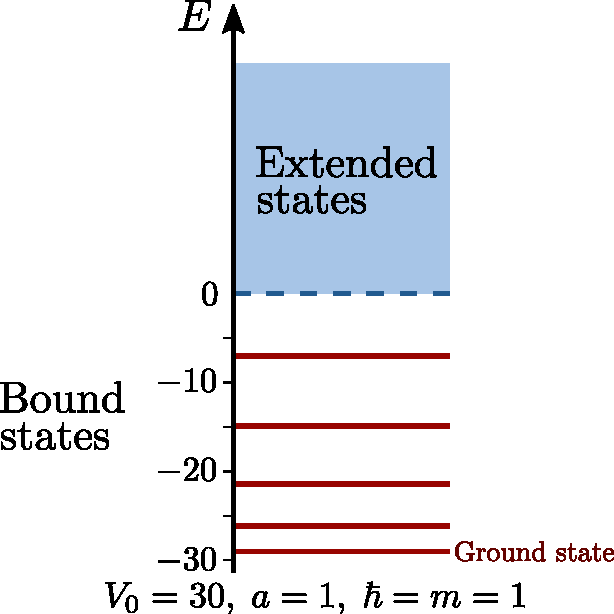
\includegraphics[width=0.4\textwidth]{boundvsextended}
\end{figure}

%% For $E \ge 0$, there is a continuum of extended states, which do not
%% have any finite normalization.  For $-V_0 < E < 0$, which is the
%% energy range ``inside'' the potential well, there exists a discrete
%% and finite set of bound states, whose wavefunctions vanish
%% exponentially outside the well and are therefore normalizable.

Many of the lessons drawn from this square well model can be
generalized to more complicated potential wells, so long as (i) the
potential at infinity is some finite value $V_{\textrm{ext}}$ and (ii)
the potential describes a ``well'' (i.e., it has some minimum value
$V_{\mathrm{min}} < V_{\textrm{ext}}$).  For energies $E \ge
V_{\textrm{ext}}$, there will exist a continuum of extended
(non-normalizable) states.  And for $V_{\mathrm{min}} < E <
V_{\textrm{ext}}$, there can exist a discrete set of bound
(normalizable) states.

There are, however, two important provisos.  The first is that the set
of bound states might be empty: i.e., a potential well can be ``too
shallow'' to support a bound state.  This is observable in the
numerical results for the square well model (see
\hyperref[sec:appendix]{Appendix A}).  An intuitive explanation is
that all quantum wavefunctions possess some ``zero-point'' energy, and
if this exceeds the well depth, bound states cannot form.  The second
proviso is that in certain cases, it turns out to be possible to have
bound states with energy $E \ge V_{\textrm{ext}}$.  These are called
``bound states in the continuum'', since they lie in the same energy
range as the continuum of extended states.  We will ignore this
phenomenon, since it happens only under special circumstances that lie
outside the scope of the present discussion.

\section{Quasi-bound states and resonances}

The bound states and extended states of the finite square well are
extremely different from each other.  But under certain circumstances,
extended states can take on characteristics that make them very
similar to bound states.  These are called \textbf{quasi-bound
  states}, and as we shall see, they play an especially important role
in scattering experiments.

An example of a potential function $V(x)$ that supports quasi-bound
states is shown below.  In the external regions, $|x| > b$, the
potential is $V(x) = V_{\textrm{ext}} = 0$.  Between $x = -b$ and $x =
b$, there is a ``wall'' of positive potential $V_1$.  Embedded in the
middle of this wall, in the region $|x| < a$, is a central well of
potential $V_0$ such that $0 < V_0 < V_1$.

\textcolor{red}{[Fig.]}

Since $V_0, V_1 > V_{\mathrm{ext}}$, we know from the discussion in
the previous section that the system does not support any bound
states, only extended states.

However, there's something intriguing about the energy range $V_0 < E
< V_1$, which are the energies of the central well.  Suppose that we
set the external potential as $V_{\mathrm{ext}} = V_1$ rather than
$V_{\mathrm{ext}} = 0$.  In that case, the central well would be able
to support bound states, which would be exponentially localized to the
vicinity of the well.  Since this scenario differs from the actual
scenario only in the value of $V_{\mathrm{ext}}$, and the bound state
wavefunctions are exponentially suppressed in the external region, it
follows that the bound states that exist for $V_{\mathrm{ext}} = V_1$
are \textit{approximate} energy eigenstates of the $V_{\mathrm{ext}} =
0$ system.

Turning this argument around, we expect our actual system (which has
$V_{\mathrm{ext}} = 0$) to possess certain extended states whose
wavefunctions look highly similar to bound states, but aren't actually
bound.

To look for evidence of this, we analyze the system using the
framework of a \textbf{scattering experiment}, of the sort described
in the previous chapter.  Let a particle be incident from the left,
with energy $E > 0$, described by the incident wavefunction
$$\psi_i(x) = \Psi_i \, e^{ik_i x}.$$
This gives rise to a scattered wavefunction $\psi_s(x)$, such that the
total wavefunction $\psi_i(x) + \psi_s(x)$ satisfies the Schr\"odinger
wave equation with energy $E$.  The scattered wavefunction must be
outgoing (see the previous chapter), so in the external region it
takes the form
$$\psi_s(x) = \Psi_i \times \begin{cases}f_- \,e^{-ik_ix}, & x < -b \\ f_+ \,e^{ik_ix}, & x > b.\end{cases}$$
The scattering amplitudes $f_+$ and $f_-$ can be computed by solving
the Schr\"odinger wave equation.  Details about the solution method
are, once again, deferred to Appendix A.  The results are shown in the
figure below (using a typical choice of model parameters:
\textcolor{red}{[???]}).

\textcolor{red}{[Fig.]}

The vertical axis in this figure is the ``scattering intensity''
$|f_+|^2 + |f_-|^2$, which is a measure of how strongly the incident
wave is scattered.  (Here, it so happens that $|f_+| = |f_-|$, due to
our potential's mirror symmetry.)  The horizontal axis is the incident
energy $E$.  Underneath the $E$ axis, we have plotted arrows
indicating the quasi-bound state energies, as obtained from a separate
calculation---these are the energies of the bound states that would
exist if $V_{\mathrm{ext}} = V_1$.

As seen in this figure, quasi-bound states coincide with strong peaks
in the scattering intensity.  This peaks are called \textbf{scattering
  resonances}.  If we examine the total wavefunction at these special
energies, we see something else that is very interesting: the
probability density $|\psi(x)|^2$ is hugely enhanced within the well
region.  An example is shown in the figure below (using $E =
\textcolor{red}{???}$, which corresponds to the lowest-energy
scattering resonance in our example system):

\textcolor{red}{[Fig.]}

The enhancement of $|\psi(x)|^2$ is explained by the aforementioned
similarity of the quasi-bound state to a bound state (which is
exponentially localized to the well region).  It is also closely
related to the phenomenon of \textbf{resonance} from classical
mechanics: if we take a mechanical system with a natural oscillation
frequency (such as a damped harmonic oscillator) and drive it at a
fixed frequency, the oscillation amplitude becomes extremely large
when the driving frequency matches the natural oscillation frequency.
Here, the quasi-bound state energy plays the role of the natural
oscillation frequency, and the incident energy $E$ plays the role of
the driving frequency.

It is hard to overstate the importance of scattering resonances for
experimental physics.  Experiments are often conducted for the express
purpose of locating and characterizing scattering resonances.  The
location of the peak tells us that the system being probed has a
quasi-bound state at that energy, while the width and shape of the
peak can be used to deduce other properties of the quasi-bound state.

%% The figure below, for instance, shows ...

\textcolor{red}{[Fig.]}

%% The above figure show two experimental plots, from completely
%% different experiments, in which resonances were

\section{General analysis of scattering resonances}

Quasi-bound states and scattering resonances are not limited to 1D;
they are equally important, if not more so, in 2D and 3D systems.  The
Green's function operator, introduced in the previous chapter,
provides a convenient and general way to study them.



\section{Decay rate of a quasi-bound state: Fermi's Golden Rule}

\section{The decay spectrum of beta particles}


\appendix
\section{The transfer matrix method}
\label{sec:appendix}


\section{Normalization of bound states and extended states}
\label{sec:normalization}

In this Appendix, we take a closer look at where bound and extended
states come from, and how they are normalized.  Imagine that instead
of taking $x \in (-\infty,\infty)$, we enclose the system in a very
large but finite box, so that $x \in [-L,L]$ where $L \gg a$.  We
impose periodic boundary conditions on the box walls, $\psi(-L) \equiv
\psi(L)$, and solve the Schr\"odinger equation for wavefunctions
normalizable within the box, such that $\int_{-L}^{L} |\psi(x)|^2 dx =
1$.  For any finite $L$, there is an infinite but discrete set of
solutions, with energies in the range $-V_0 <E < \infty$.

We now examine how the solutions vary upon increasing $L$.

\textcolor{red}{[Fig.]}





\section*{Exercises}

\begin{enumerate}
\item Phase shift under scattering resonance

\item Classical driven oscillator analogy  
\end{enumerate}




\section*{Further Reading}

\begin{itemize}
\item Bransden \& Joachain, \S4.4, 9.2--9.3, 13.4
\item Sakurai, \S5.6, 7.7--7.8

\end{itemize}


\end{document}


%% For decades after the discovery of quantum mechanics, the quantum
%% double-slit experiment was just a ``thought experiment'', meant to
%% illustrate the features of quantum mechanics that had been uncovered
%% by other, more complicated experiments.  Nowadays, the most convenient
%% way to do the experiment is with light, using single-photon sources
%% and single-photon detectors.  Quantum interference has also been
%% demonstrated experimentally using electrons, neutrons, and even
%% large-scale particles such as buckyballs.
